\chapter{Implementation}
\label{chap:impl}

In this chapter we describe the implementation of our framework from Chapter~\ref{chap:approach}. Our implementation comprises a Python library kairo and a dashboard built on top of kairo. Both are placed in the public repository of this thesis\footnote{\url{https://github.com/boraderen/thesis}}. We introduce the structure of the code and design choices of the implementation.

An LLM supports the analysis in two ways (Figure~\ref{fig:impl:ai}). It is not a further step of the pipeline and does not do any computations.
\begin{itemize}
	\item \emph{Analysis of results:} The Copilot of the dashboard is used to interpret the results of the pipelines. Its main purpose is to assist the user. The Copilot allows the user to chat with an LLM on the analysis by sharing the results of the computations of the pipelines, plots and textual abstractions (Section~\ref{sec:impl:dashboard:copilot}).
	\item \emph{Agentic analysis:} An agent executes the pipeline itself by using kairo and tests different configurations (Section~\ref{sec:impl:kairo:agent}).
\end{itemize}
Thus, this chapter addresses the research goals~\ref{item:intro:rg_library} and~\ref{item:intro:rg_dashboard}.

\begin{figure}[tb]
	\centering
	\begin{tikzpicture}[font=\small, >={Stealth},
			box/.style={draw, rounded corners=2pt, fill=black!6, align=center, minimum height=1.1cm},
			head/.style={anchor=west, font=\small\bfseries},
			label/.style={font=\footnotesize}]
		% use case (a): the results of a pipeline go to the llm as text abstractions and plots
		\node[head] at (-0.1, 3.75) {(a) Analysis of the results};
		\node[box, text width=2.1cm] (results) at (1.1, 2.2) {Results of the pipeline (Figure~\ref{fig:approach:overview})};
		\node[box, text width=2.9cm] (abstractions) at (4.3, 2.2) {Text \mbox{abstractions} and plots};
		\node[box, text width=1.6cm] (llm) at (7.2, 2.2) {LLM};
		\node[box, text width=2.2cm, minimum height=0.8cm] (prompt) at (7.2, 3.75) {System prompt};
		\node[box, text width=1.6cm] (user) at (10.9, 2.2) {User};
		\draw[->] (results) -- (abstractions);
		\draw[->] (abstractions) -- (llm);
		\draw[->] (prompt) -- (llm);
		\draw[->] ([yshift=0.25cm]user.west) -- node[label, above] {question} ([yshift=0.25cm]llm.east);
		\draw[->] ([yshift=-0.25cm]llm.east) -- node[label, below] {answer} ([yshift=-0.25cm]user.west);
		% use case (b): an analysis agent runs the pipeline itself with the functions of kairo
		\node[head] at (-0.1, 0.55) {(b) Analysis agent};
		\node[box, text width=4.3cm] (kairo) at (2.3, -0.6) {kairo: the steps of the pipeline, plots and text abstractions as functions};
		\node[box, text width=1.6cm] (agent) at (7.2, -0.6) {Analysis agent (LLM)};
		\node[box, text width=1.6cm] (user2) at (10.9, -0.6) {User};
		\draw[->] ([yshift=0.25cm]agent.west) -- node[label, above] {calls} ([yshift=0.25cm]kairo.east);
		\draw[->] ([yshift=-0.25cm]kairo.east) -- node[label, below] {results} ([yshift=-0.25cm]agent.west);
		\draw[->] ([yshift=0.25cm]user2.west) -- node[label, above] {task} ([yshift=0.25cm]agent.east);
		\draw[->] ([yshift=-0.25cm]agent.east) -- node[label, below] {report} ([yshift=-0.25cm]user2.west);
	\end{tikzpicture}
	\caption[Two uses of an LLM on top of the framework]{%
		Two uses of an LLM on top of the framework. Boxes are components, and arrows show what they pass on.
		(a)~The results of a pipeline reach the LLM as text abstractions and plots, and a system prompt instructs the LLM. The user and the LLM interact in a chat.
		(b)~An analysis agent runs the pipeline itself by calling the functions of kairo and reads their results.}
	\label{fig:impl:ai}
\end{figure}

Section~\ref{sec:impl:kairo} presents kairo and our skill \texttt{kairo-drift-analyst} for the agentic analysis.
Section~\ref{sec:impl:dashboard} presents our dashboard and the Kairo Copilot.

\section{Kairo}
\label{sec:impl:kairo}
kairo is a Python library that implements the four steps of the framework for all three perspectives. The documentation\footnote{\url{https://boraderen.github.io/thesis/}} describes the approach, gives a quickstart and explains all functions. The nine notebooks\footnote{\url{https://github.com/boraderen/thesis/tree/main/notebooks/kairo_examples}} introduce the pipelines for each combination of perspectives and clustering algorithms. In the repository root, \texttt{uv sync} installs kairo with dependencies.

\subsection{Running the Pipeline in Python}
\label{sec:impl:kairo:pipeline}
Our implementation follows three main design principles:

\begin{itemize}
	\item \emph{Modular function structure:} Each step is a function, e.g., \texttt{compute\_features\_inter}, \texttt{standardize}, \texttt{compute\_kmeans} and \texttt{compute\_drift\_signal}. Their parameters are the parameters of Chapter~\ref{chap:approach}, e.g., the feature groups, the feature window or the divergence.
	\item \emph{DataFrames:} The log, the feature matrices, the states and the drift signal are pandas DataFrames (Figure~\ref{fig:impl:workflow}). The meta columns \texttt{case:concept:name} and \texttt{time:timestamp} travel along through all steps, but do not enter the computations. Thus, steps such as scaling and PCA can be skipped, and own features can replace the feature groups of kairo.
	\item \emph{Results as plot and text abstractions}: For the results of each step, the functions \texttt{plot\_*} create plots, and the functions \texttt{abstract\_*} summarize them as text for an LLM (Section~\ref{sec:impl:kairo:agent}).
\end{itemize}

These design choices have two advantages and two disadvantages:
\begin{itemize}
	\item \emph{Flexibility:} Steps can be skipped or exchanged, e.g., by own features or by an own clustering whose states enter the drift signal like the states of kairo.
	\item \emph{Traceability:} Each intermediate result is a DataFrame with a plot and a text abstraction, so the user can check each step.
	\item \emph{Large hyperparameter space:} The user chooses the features, the windows, the scaling, the PCA cut, the clustering algorithm with its parameters and the drift signal. This hyperparameter space is too large to test all configurations, and an unsuitable configuration can produce misleading drift signals. The Copilot and the analysis agent help the user to find a suitable configuration.
	\item \emph{Computational effort:} kairo keeps the log and the feature matrices in memory. For large logs, single steps become slow, e.g., the k-distances for DBSCAN on the intra-case features, which have one row per event.
\end{itemize}


\begin{figure}[tbp]
	\centering
	% workflow of kairo for one perspective: every arrow is a function, every symbol its output
\begin{tikzpicture}[font=\small, >={Stealth},
		wfstep/.style={->, thick},
		wffn/.style={anchor=west, font=\footnotesize, align=left},
		wfdata/.style={anchor=east, font=\footnotesize, align=right},
		wfgrid/.style={step=0.2, black!35, very thin}]
	\definecolor{wfA}{RGB}{0,114,178}
	\definecolor{wfB}{RGB}{230,159,0}
	\definecolor{wfC}{RGB}{0,158,115}
	\def\wftype#1{{\color{black!55}#1}}
	% event log, a database
	\begin{scope}[shift={(0,0)}]
		\fill[black!6] (-0.7,-0.35) rectangle (0.7,0.35);
		\fill[black!6] (0,-0.35) ellipse (0.7 and 0.15);
		\draw (-0.7,0.35) -- (-0.7,-0.35);
		\draw (0.7,0.35) -- (0.7,-0.35);
		\draw (-0.7,-0.35) arc (180:360:0.7 and 0.15);
		\draw (-0.7,-0.12) arc (180:360:0.7 and 0.15);
		\draw (-0.7,0.12) arc (180:360:0.7 and 0.15);
		\filldraw[fill=black!15] (0,0.35) ellipse (0.7 and 0.15);
	\end{scope}
	\node[wfdata] at (-1.7,0) {Event log\\\wftype{XES or CSV file}};
	% log, one row per event
	\begin{scope}[shift={(0,-1.8)}]
		\fill[black!15] (-1.0,0.2) rectangle (1.0,0.4);
		\draw[wfgrid] (-1.0,-0.4) grid (1.0,0.4);
		\draw (-1.0,-0.4) rectangle (1.0,0.4);
	\end{scope}
	\node[wfdata] at (-1.7,-1.8) {Log\\one row per event\\\wftype{\texttt{DataFrame}}};
	% feature matrix, wide
	\begin{scope}[shift={(0,-3.6)}]
		\fill[black!20] (-1.4,-0.4) rectangle (-1.2,0.4);
		\draw[wfgrid] (-1.4,-0.4) grid (1.4,0.4);
		\draw (-1.4,-0.4) rectangle (1.4,0.4);
	\end{scope}
	\node[wfdata] at (-1.7,-3.6) {Feature matrix $X$\\$m \times n$\\\wftype{\texttt{DataFrame}}};
	% scaled matrix, same size
	\begin{scope}[shift={(0,-5.4)}]
		\fill[wfA!12] (-1.2,-0.4) rectangle (1.4,0.4);
		\fill[black!20] (-1.4,-0.4) rectangle (-1.2,0.4);
		\draw[wfgrid] (-1.4,-0.4) grid (1.4,0.4);
		\draw (-1.4,-0.4) rectangle (1.4,0.4);
	\end{scope}
	\node[wfdata] at (-1.7,-5.4) {Scaled matrix\\$m \times n$\\\wftype{\texttt{DataFrame}}};
	% reduced matrix, narrow
	\begin{scope}[shift={(0,-7.2)}]
		\fill[wfA!25] (-0.2,-0.4) rectangle (0.4,0.4);
		\fill[black!20] (-0.4,-0.4) rectangle (-0.2,0.4);
		\draw[wfgrid] (-0.4,-0.4) grid (0.4,0.4);
		\draw (-0.4,-0.4) rectangle (0.4,0.4);
	\end{scope}
	\node[wfdata] at (-1.7,-7.2) {Reduced matrix $Z$\\$m \times d$, $d \le n$\\\wftype{\texttt{DataFrame}}};
	% states, clusters of rows
	\begin{scope}[shift={(0,-9.0)}]
		\foreach \x/\y in {-0.95/0.1, -0.8/0.25, -0.7/0.02, -0.85/-0.12, -0.6/0.18}
			\fill[wfA] (\x,\y) circle (0.055);
		\foreach \x/\y in {-0.1/-0.2, 0.05/-0.05, 0.12/-0.25, -0.05/-0.32, 0.2/-0.12}
			\fill[wfB] (\x,\y) circle (0.055);
		\foreach \x/\y in {0.65/0.2, 0.8/0.05, 0.9/0.25, 0.75/0.32, 1.0/0.12}
			\fill[wfC] (\x,\y) circle (0.055);
		\draw[densely dashed, black!50] (-0.78,0.08) ellipse (0.3 and 0.28);
		\draw[densely dashed, black!50] (0.04,-0.18) ellipse (0.3 and 0.24);
		\draw[densely dashed, black!50] (0.82,0.18) ellipse (0.3 and 0.24);
	\end{scope}
	\node[wfdata] at (-1.7,-9.0) {States\\one per row of $Z$\\\wftype{\texttt{DataFrame}}};
	% state distributions, shares per signal window
	\begin{scope}[shift={(0,-10.8)}]
		\foreach \x/\a/\b in {-1.0/0.5/0.3, -0.6/0.48/0.32, -0.2/0.52/0.28, 0.2/0.12/0.24, 0.6/0.1/0.26, 1.0/0.14/0.22} {
			\fill[wfA] (\x-0.14,-0.4) rectangle (\x+0.14,-0.4+\a);
			\fill[wfB] (\x-0.14,-0.4+\a) rectangle (\x+0.14,-0.4+\a+\b);
			\fill[wfC] (\x-0.14,-0.4+\a+\b) rectangle (\x+0.14,0.4);
		}
	\end{scope}
	\node[wfdata] at (-1.7,-10.8) {State distributions\\one per signal window\\\wftype{\texttt{DataFrame}}};
	% drift signal, a spike
	\begin{scope}[shift={(0,-12.6)}]
		\draw[->, black!60] (-1.25,-0.4) -- (1.3,-0.4);
		\draw[->, black!60] (-1.2,-0.45) -- (-1.2,0.45);
		\draw[wfA, thick] (-1.1,-0.32) -- (-0.8,-0.3) -- (-0.5,-0.33) -- (-0.2,-0.31) -- (0.0,0.35) -- (0.2,-0.3) -- (0.5,-0.32) -- (0.8,-0.31) -- (1.1,-0.33);
	\end{scope}
	\node[wfdata] at (-1.7,-12.6) {Drift signal\\one score per signal window\\\wftype{\texttt{DataFrame}}};
	% the functions between the outputs
	\foreach \y/\fn in {
			-0.9/{\texttt{kairo.read\_log}},
			-2.7/{\texttt{kairo.compute\_features\_intra}, \texttt{\_resource} or \texttt{\_inter}},
			-4.5/{\texttt{kairo.standardize} (optional)},
			-6.3/{\texttt{kairo.compute\_pca} \wftype{(\texttt{PCA})}, then\\\texttt{kairo.apply\_pca} (optional)},
			-8.1/{\texttt{kairo.compute\_som}, \texttt{\_kmeans} or \texttt{\_dbscan}\\\wftype{(\texttt{MiniSom}, \texttt{KMeans} or \texttt{DBSCAN})}, then \texttt{kairo.get\_*\_states}},
			-9.9/{\texttt{kairo.compute\_state\_distributions}},
			-11.7/{\texttt{kairo.compute\_drift\_signal}}} {
		\draw[wfstep] (0,\y+0.4) -- (0,\y-0.4);
		\node[wffn] at (0.2,\y) {\fn};
	}
\end{tikzpicture}

	\caption[Workflow of kairo]{%
		Workflow of kairo for one perspective. Each arrow is a function of kairo that takes the output above it and returns the output below it. Gray text gives the type of each output: except for the event log, every output is a pandas DataFrame, and fitting PCA or a clustering returns the fitted model, which the next function applies. The gray first column of the matrices stands for the meta columns, which travel along but do not enter the computations.}
	\label{fig:impl:workflow}
\end{figure}

\subsection{Agentic Analysis}
\label{sec:impl:kairo:agent}
Since kairo consists of small, documented functions with DataFrames as input and output, an analysis agent can run the pipeline itself (Figure~\ref{fig:impl:ai}). By an analysis agent, we mean an LLM with tools to read files and to run code. The agent calls the functions of kairo, combines them, tests configurations and computes own features if needed.

The agent reads the results as text abstractions. According to \textcite{berti2024abstractions}, a complete event log cannot be given to an LLM as a prompt due to its size. Therefore, they implement textual abstractions of process mining artifacts, e.g., of event logs and process models, in PM4Py. Similarly, each function \texttt{abstract\_*} of kairo summarizes one result as text. An abstraction only names what matters for the interpretation, e.g., the signal windows with the highest drift scores. Figure~\ref{fig:impl:abstraction} shows an example of an abstraction.

\begin{figure}[tb]
	\centering
	\begin{minipage}{0.95\textwidth}
		\footnotesize
		% generated by notebooks/thesis, do not edit by hand
\begin{verbatim}
Drift signal: for every signal window, the KL divergence between its state
distribution and the previous signal window, the drift score of the signal window.
54 signal windows from 2019-12-26 00:00:00+00:00 to 2020-12-31 00:00:00+00:00.
Drift scores: median 0.074, mean 0.678, highest 14.958.
The signal windows with the highest drift scores:
- signal window starting 2020-10-01 00:00:00+00:00: 14.958
- signal window starting 2020-02-20 00:00:00+00:00: 2.550
- signal window starting 2020-08-27 00:00:00+00:00: 2.550
- signal window starting 2020-09-10 00:00:00+00:00: 2.550
- signal window starting 2020-12-31 00:00:00+00:00: 1.946
\end{verbatim}

	\end{minipage}
	\caption[Text abstraction of a drift signal]{%
		Text abstraction of the inter-case drift signal of the running example $L_3$ with signal windows of one week and the previous signal window as reference, as the LLM reads it. Long lines are wrapped. The abstraction names the divergence and the reference, summarizes the 54 drift scores and lists the five signal windows with the highest drift scores.}
	\label{fig:impl:abstraction}
\end{figure}

Our skill \texttt{kairo-drift-analyst}\footnote{\url{https://github.com/boraderen/thesis/tree/main/skills/kairo-drift-analyst}} gives an agent the instructions for such an analysis. The prompt names the event log and the task, e.g., to find the drift points and their perspectives. The agent reads the thesis and the documentation of kairo, runs and compares configurations on its own and reports the drifts with their perspectives, modes and what changed. For each perspective, it reports a configuration with a threshold on the drift scores.

\section{Dashboard}
\label{sec:impl:dashboard}
Our dashboard\footnote{\url{https://thesis-kairo-dashboard.streamlit.app/}} is a Streamlit app built on top of kairo. In the repository root, \texttt{uv run streamlit run dashboard/app.py} starts the dashboard locally. The sidebar lists its pages: the upload page, four pages for each perspective and the Copilot.

\subsection{Running the Pipeline in the Dashboard}
\label{sec:impl:dashboard:pipeline}
On the upload page, the user uploads an event log as an XES or CSV file of up to 1~GB. By clicking on the column headers, the user assigns the columns to their roles, e.g., the case identifier, the activity and the timestamp. Then, the user picks the case attributes for the inter-case features and states whether each one is numerical or categorical.

Each perspective has four pages, one for each step: Features, PCA, States \& Trajectories and Drift Signal. In the sidebar, the user chooses the parameters of a step, e.g., the clustering algorithm and its parameters in Figure~\ref{fig:impl:dashboard_states}. Each page shows the results with the plots and tables of kairo:
\begin{itemize}
	\item \emph{States:} The page shows the clustering measures of Section~\ref{sec:prelim:cluster_eval} as well as the colors of the states and the distances between them (Figure~\ref{fig:impl:dashboard_states}). It also compares the state frequencies of two date ranges, e.g., before and after a suspected drift.
	\item \emph{Trajectories:} In the intra-case perspective, the page shows the trajectory of a single case and the trajectories of all cases in a date range. In the resource and inter-case perspectives, it shows the trajectory of the log with a table of its visits (Figure~\ref{fig:impl:dashboard_trajectory}).
	\item \emph{Drift signal:} The page shows the drift signal and the state distribution of each signal window (Figure~\ref{fig:impl:dashboard_drift}).
\end{itemize}

The user tries out configurations step by step and computes the perspectives one after another. This follows the human-in-the-loop process of \textcite{barbonjunior2018framework}, in which a human observes the emergence of drifts over time and adjusts the hyperparameters.

\begin{figure}[tbp]
	\centering
	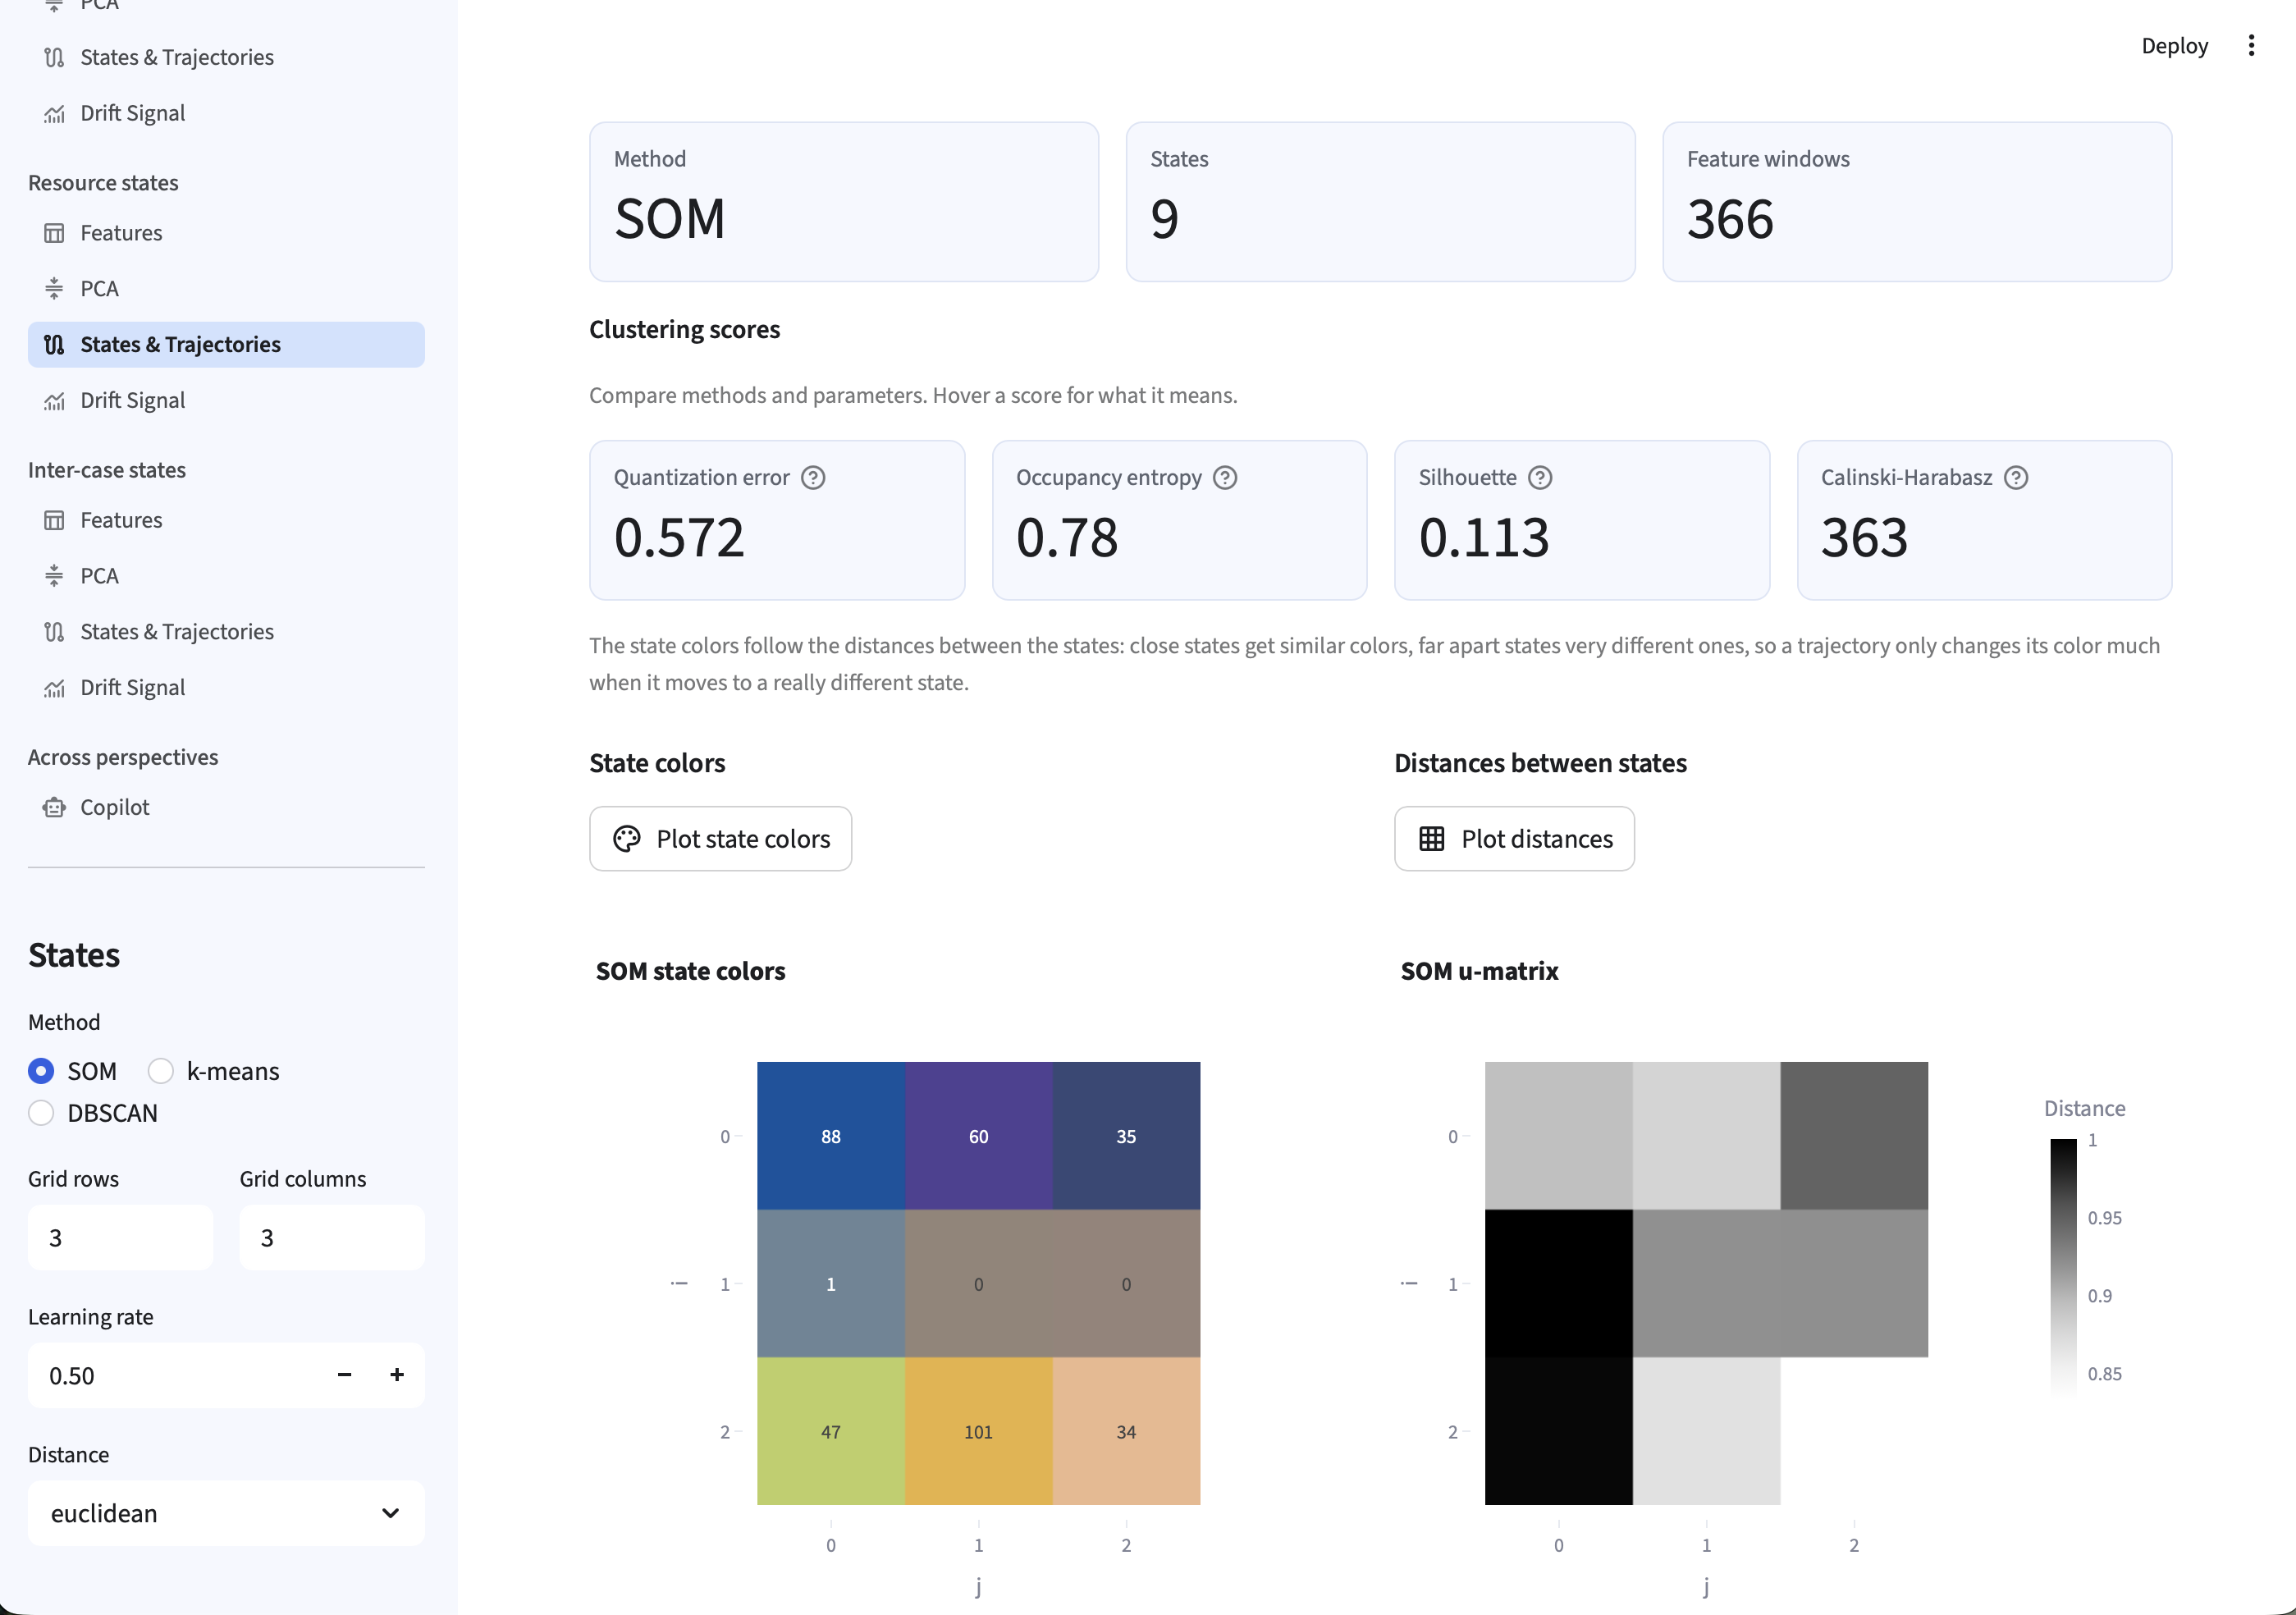
\includegraphics[width=\textwidth]{figures/dashboard/states}
	\caption[States page of the dashboard]{%
		Upper part of the States \& Trajectories page of the dashboard for the resource perspective of the running example $L_3$. The 366 feature windows of one day have the feature groups \texttt{res\_events}, \texttt{res\_cases} and \texttt{act\_res\_shares}. They are min-max scaled and reduced to 10 principal components, which explain 95.2\% of the variance. In the sidebar, the user chooses a $3 \times 3$ SOM. The page shows the clustering measures, the color of each cell with its number of feature windows and the U-matrix. Cells are counted from 0. The cells $(2, 0)$ to $(2, 2)$ hold the 182 days before the reassignment drift, and the cells $(0, 0)$ to $(0, 2)$ the 183 days after it. Since each process version spreads over three close cells, the silhouette is only 0.113.}
	\label{fig:impl:dashboard_states}
\end{figure}

\begin{figure}[tbp]
	\centering
	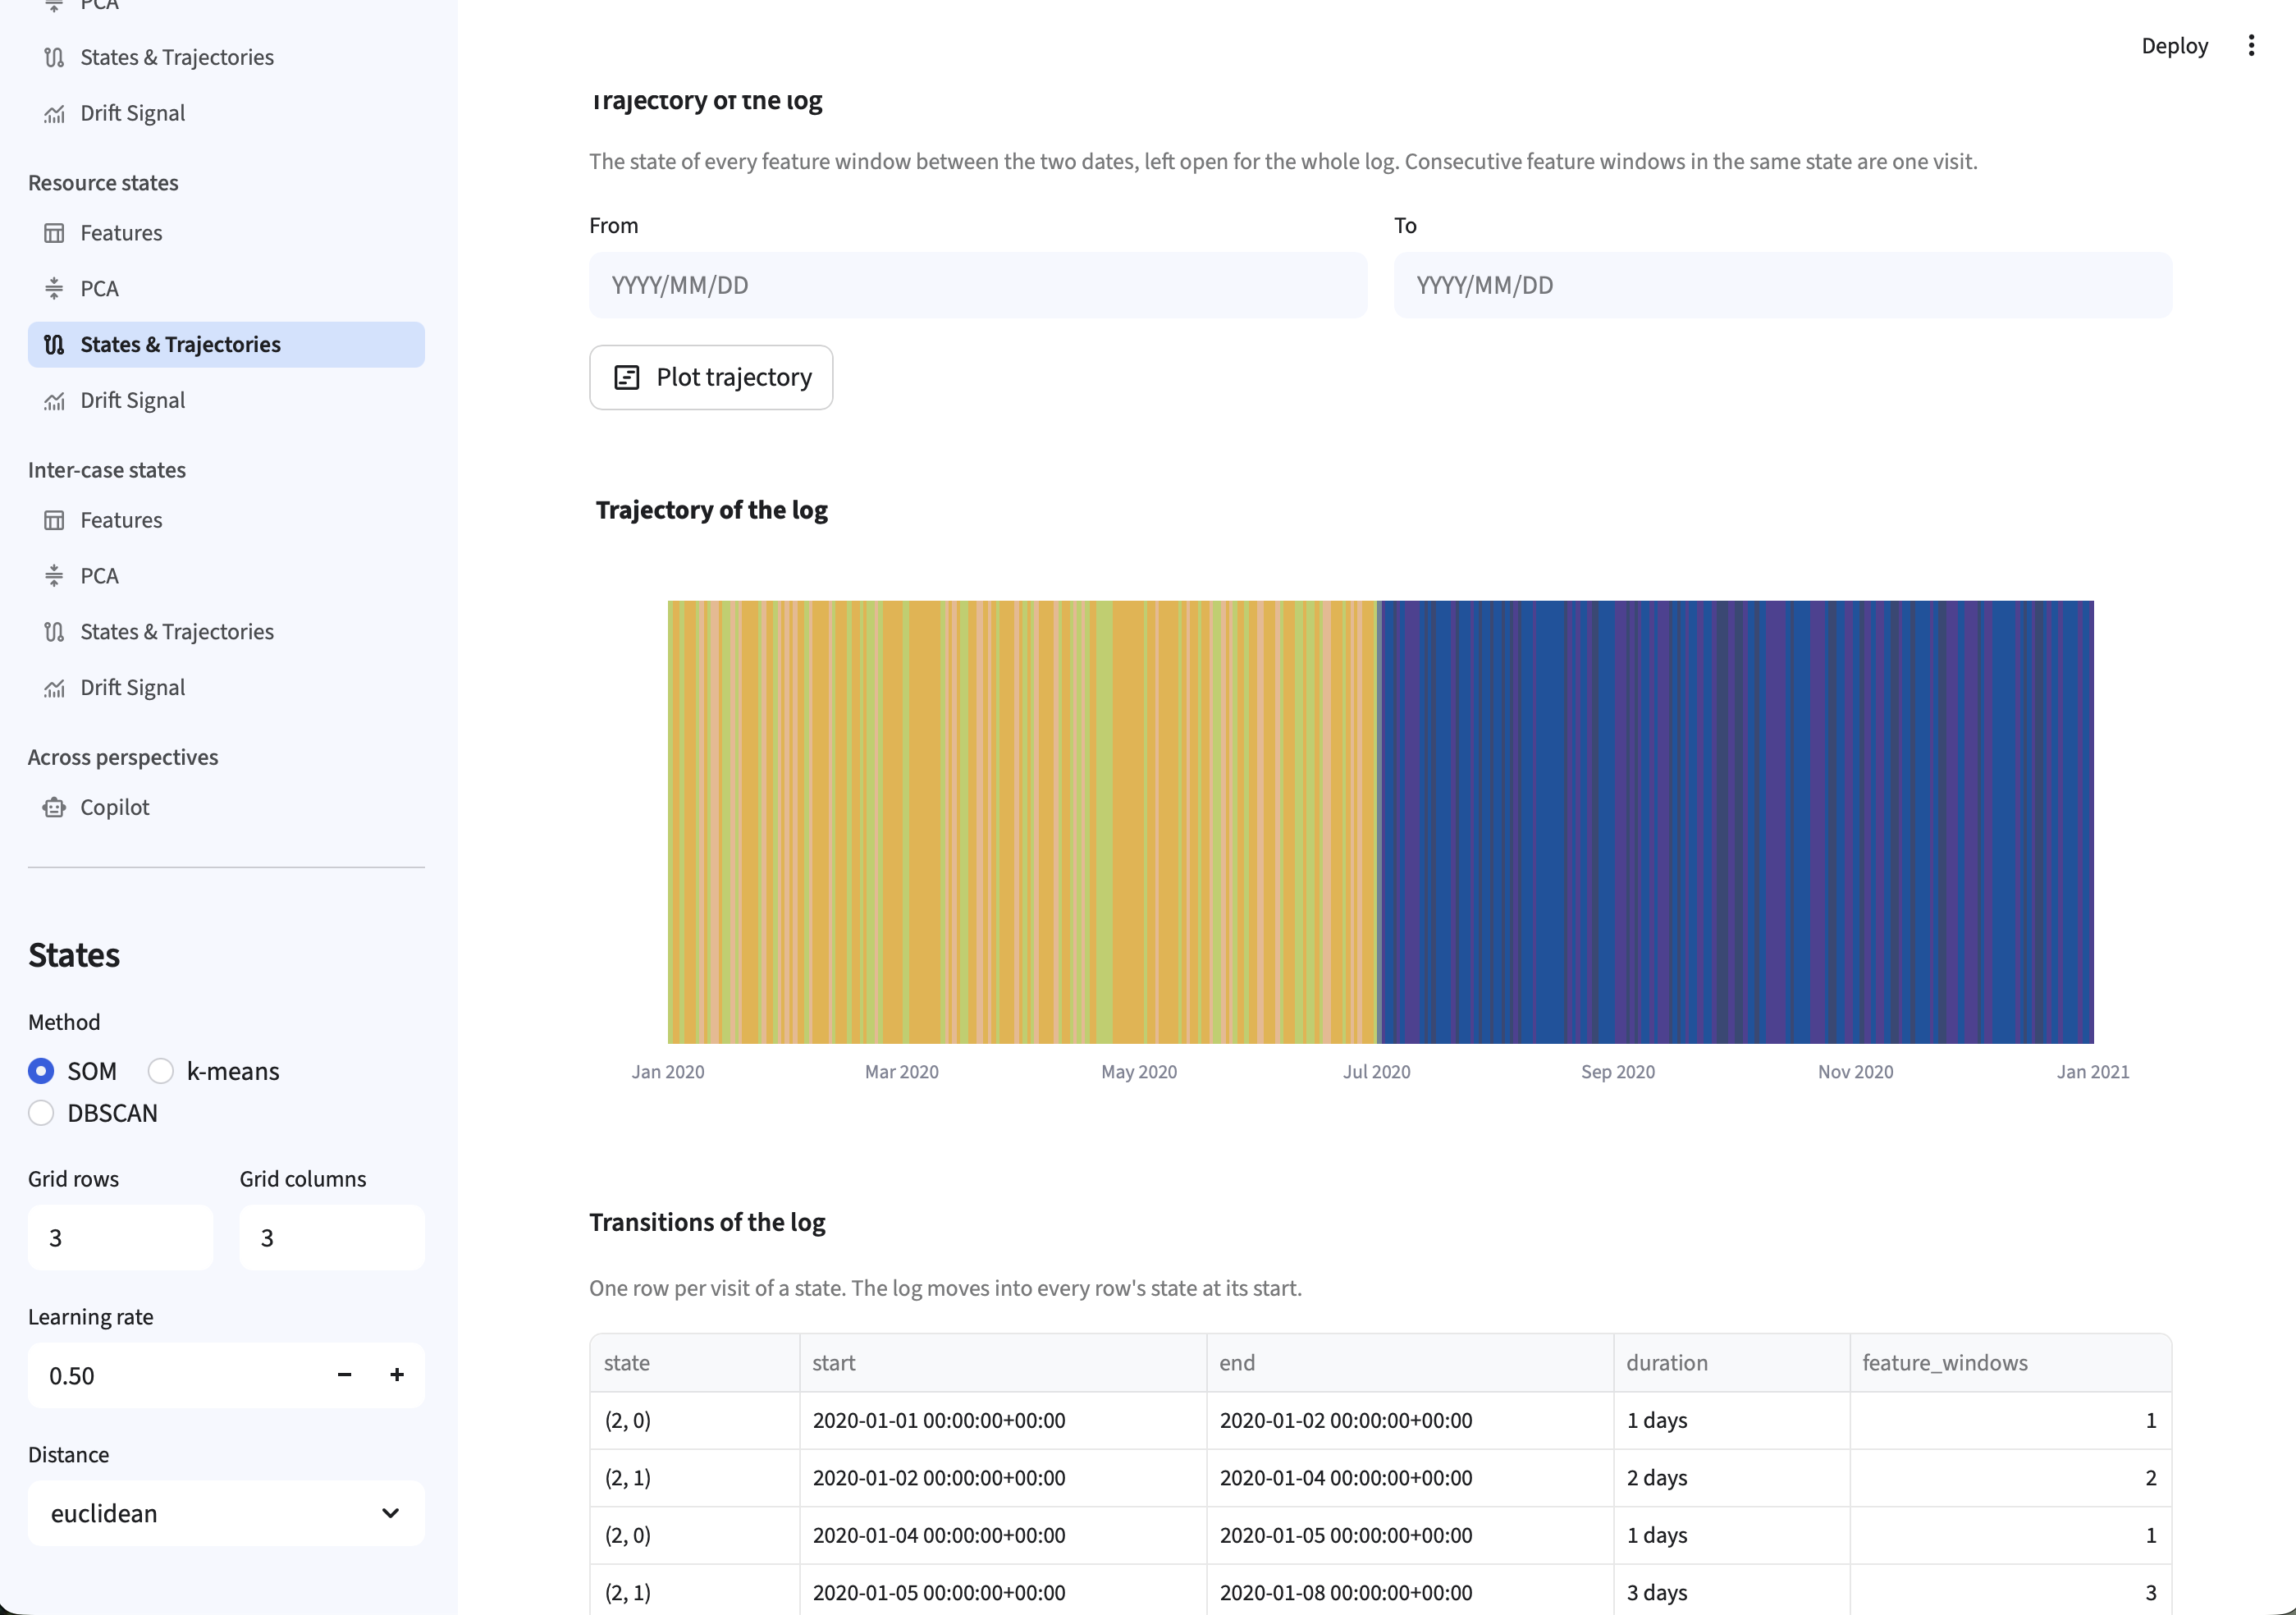
\includegraphics[width=\textwidth]{figures/dashboard/trajectory}
	\caption[Trajectory of the log in the dashboard]{%
		Lower part of the States \& Trajectories page of Figure~\ref{fig:impl:dashboard_states}. Without dates, the user plots the trajectory of the whole log. Each stripe is a feature window in the color of its state. At the reassignment drift on July~1, 2020, the colors change from yellow and orange to blue and purple. The table lists each visit of a state with its start, end, duration and number of feature windows.}
	\label{fig:impl:dashboard_trajectory}
\end{figure}

\begin{figure}[tbp]
	\centering
	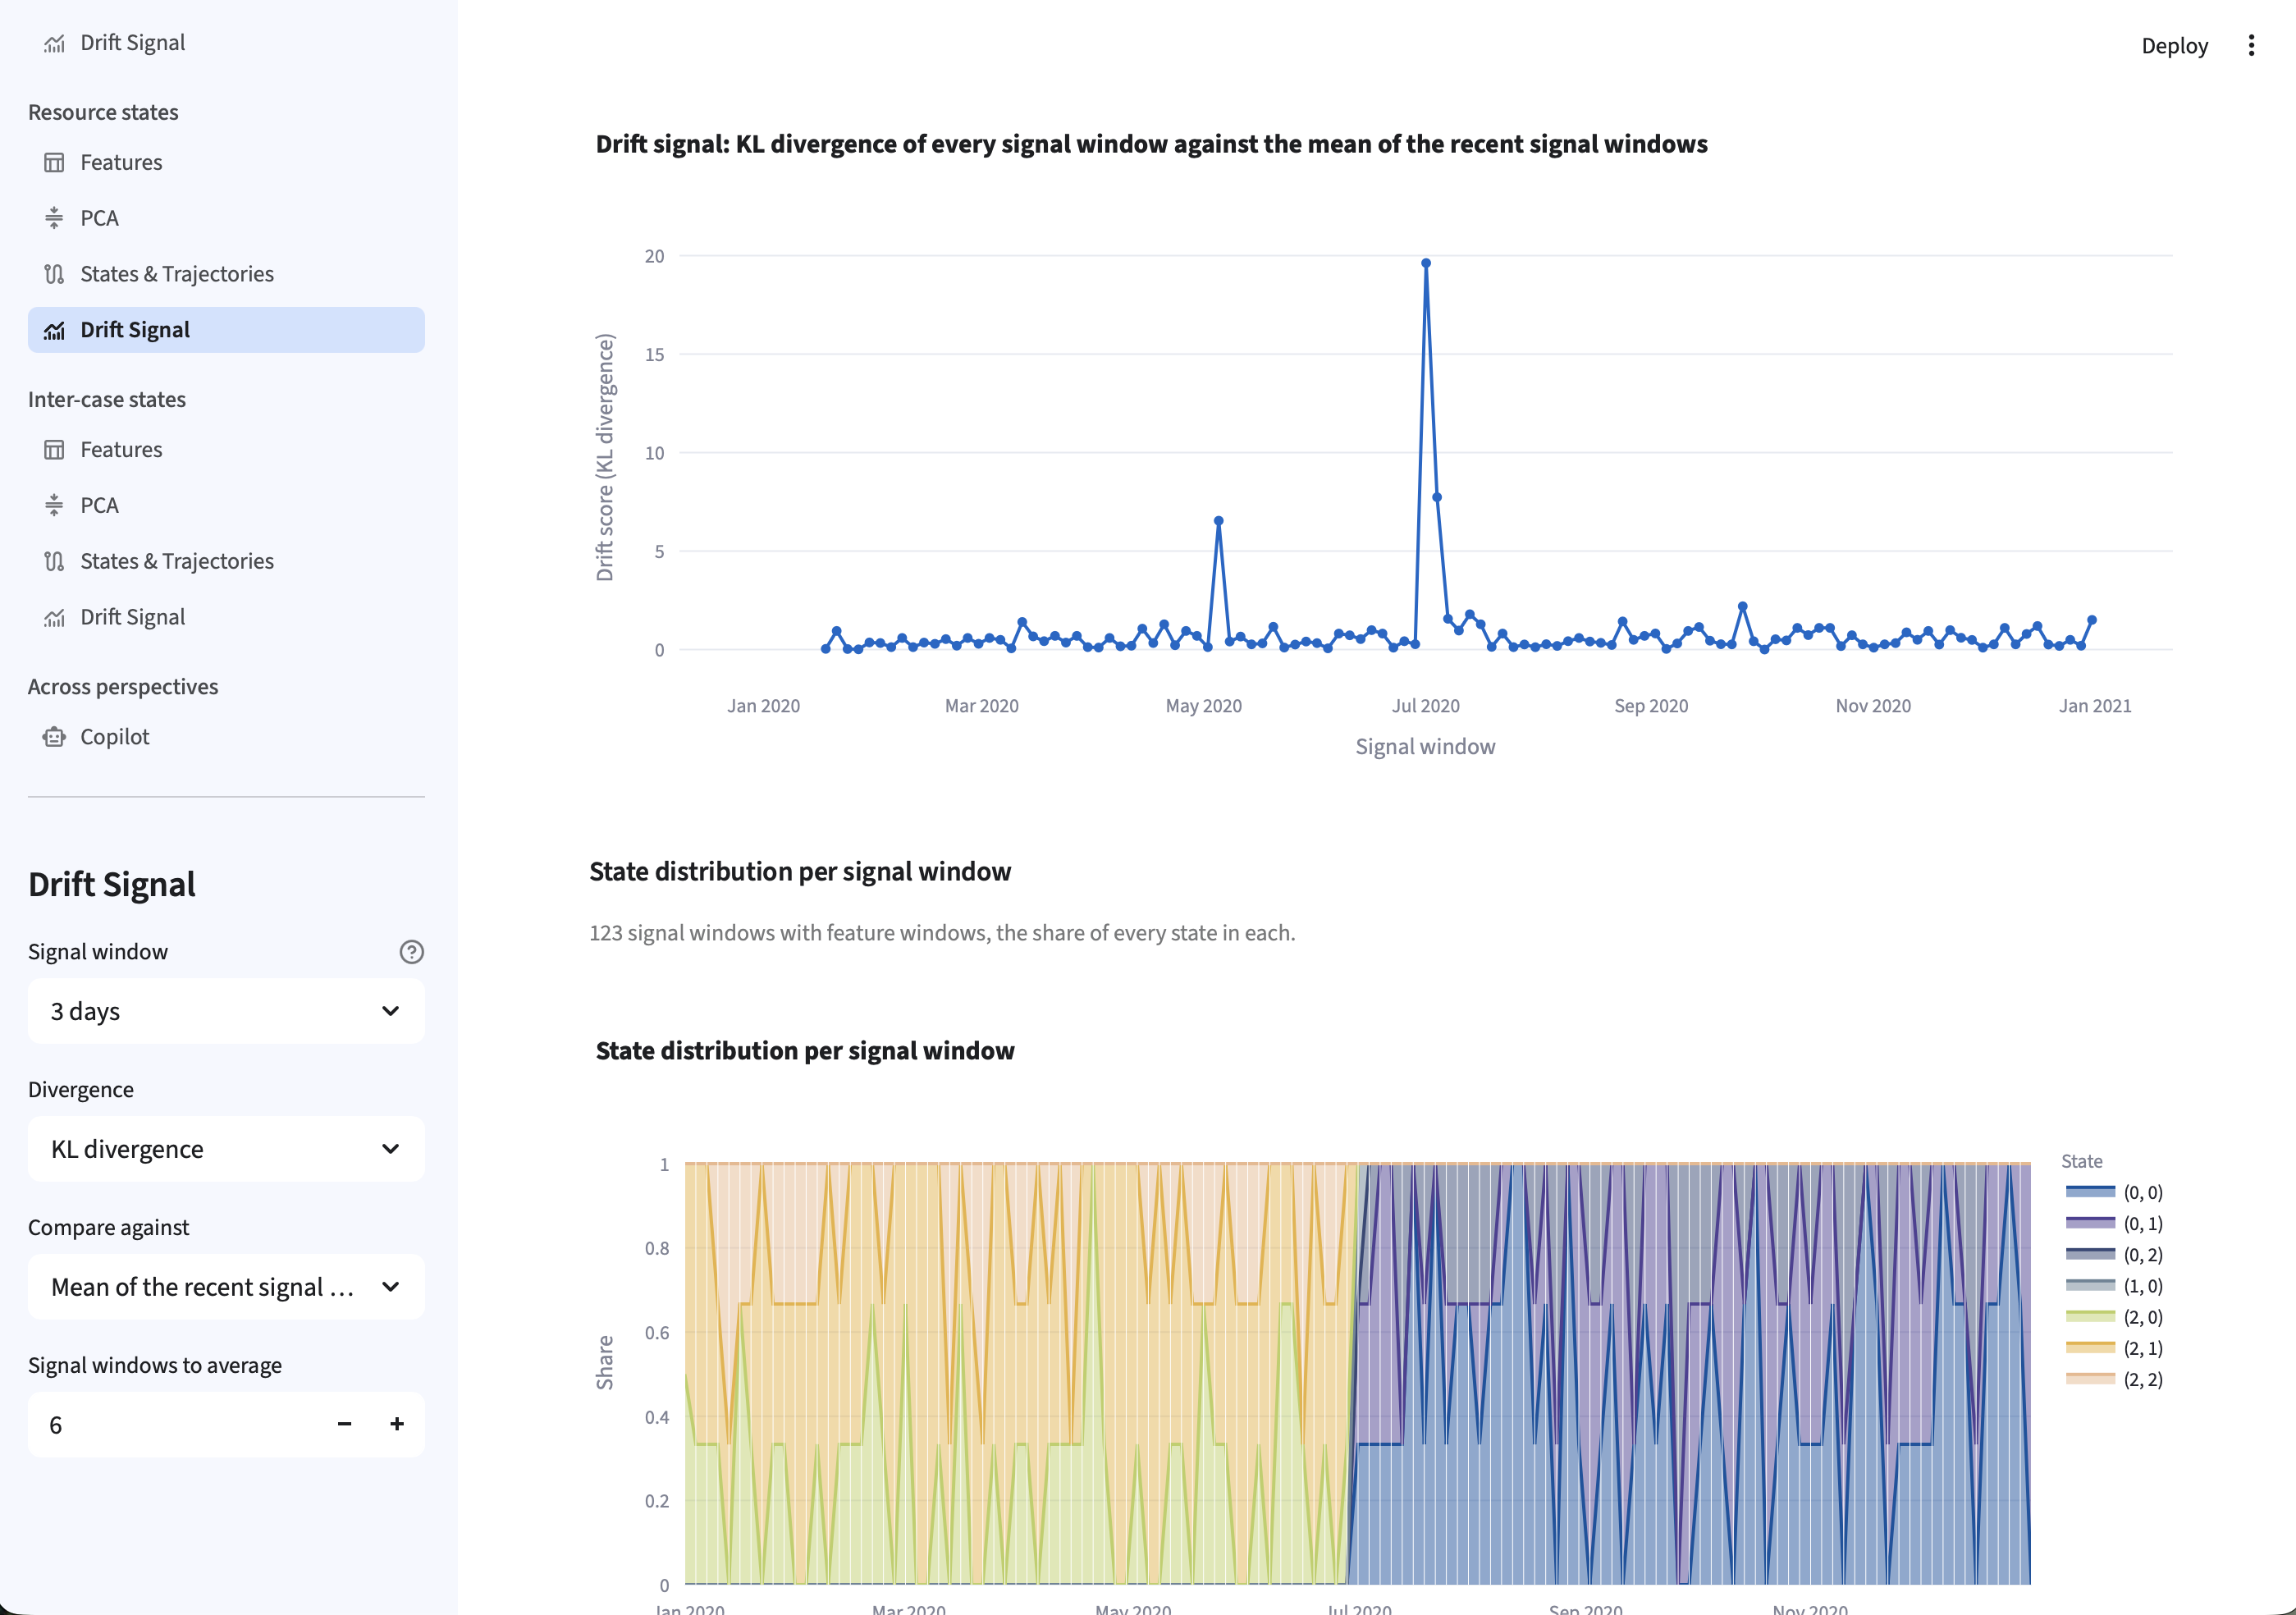
\includegraphics[width=\textwidth]{figures/dashboard/drift_signal}
	\caption[Drift signal page of the dashboard]{%
		Drift Signal page of the dashboard for the resource states of Figure~\ref{fig:impl:dashboard_states}. In the sidebar, the user chooses signal windows of three days, the KL divergence and the mean of the six previous signal windows as reference. The drift signal reaches its highest drift score of 19.62 in the signal window from July~1, 2020, which contains the reassignment drift. The smaller spike of 6.54 in the signal window from May~5 comes from state $(2, 2)$, which does not occur in the six previous signal windows. Below, the state distributions of the 123 signal windows show the change from the cells of row~2 to the cells of row~0.}
	\label{fig:impl:dashboard_drift}
\end{figure}

\subsection{Kairo Copilot}
\label{sec:impl:dashboard:copilot}
Kairo Copilot is the page of the dashboard on which an LLM analyzes the results together with the user (Figure~\ref{fig:impl:ai}). We see the Copilot as an extension of our framework and not as a step of the pipeline. It computes neither states nor drift signals, but interprets the results of the pipeline. The user picks the abstractions and plots of all steps computed so far, which the LLM receives, and asks questions (Figure~\ref{fig:impl:copilot}). The analysis is interactive: the user asks follow-up questions and requests further steps. In this way, the LLM supports the characterization of a drift (\ref{item:intro:rq_characterization}).
\begin{itemize}
	\item \emph{LLM connector:} The class \texttt{LLMConnector} of kairo has connectors for Claude and for OpenAI-compatible APIs and supports custom providers. The function \texttt{create\_messages} brings the abstractions and the plots, which are attached as images, into the message format of the provider.
	\item \emph{System prompt:} The default system prompt of kairo explains the method, the feature groups and the strengths and limits of each perspective to the LLM. It instructs the LLM to only use the shared results and never to invent numbers. Further, it tells the LLM to judge the configuration before the drift signal and to stay skeptical of drift signals that contradict each other.
	\item \emph{Chat history:} The Copilot keeps the chat history and sends it with each question, so the LLM remembers earlier questions and the results that the user shared.
\end{itemize}
In Figure~\ref{fig:impl:copilot}, the model Qwen3-VL-30B-A3B-Thinking runs as a custom provider on the GPU cluster of the Chair of Process and Data Science (PADS). With the abstractions and plots of the resource perspective of Figures~\ref{fig:impl:dashboard_states} to~\ref{fig:impl:dashboard_drift}, it names the reassignment drift in the signal window from July~1, 2020. However, an LLM can hallucinate and interpret results in a misleading way. Therefore, we suggest using it as an assistant in a human-in-the-loop analysis and staying skeptical of its claims (Chapter~\ref{chap:discussion}).

\begin{figure}[tbp]
	\centering
	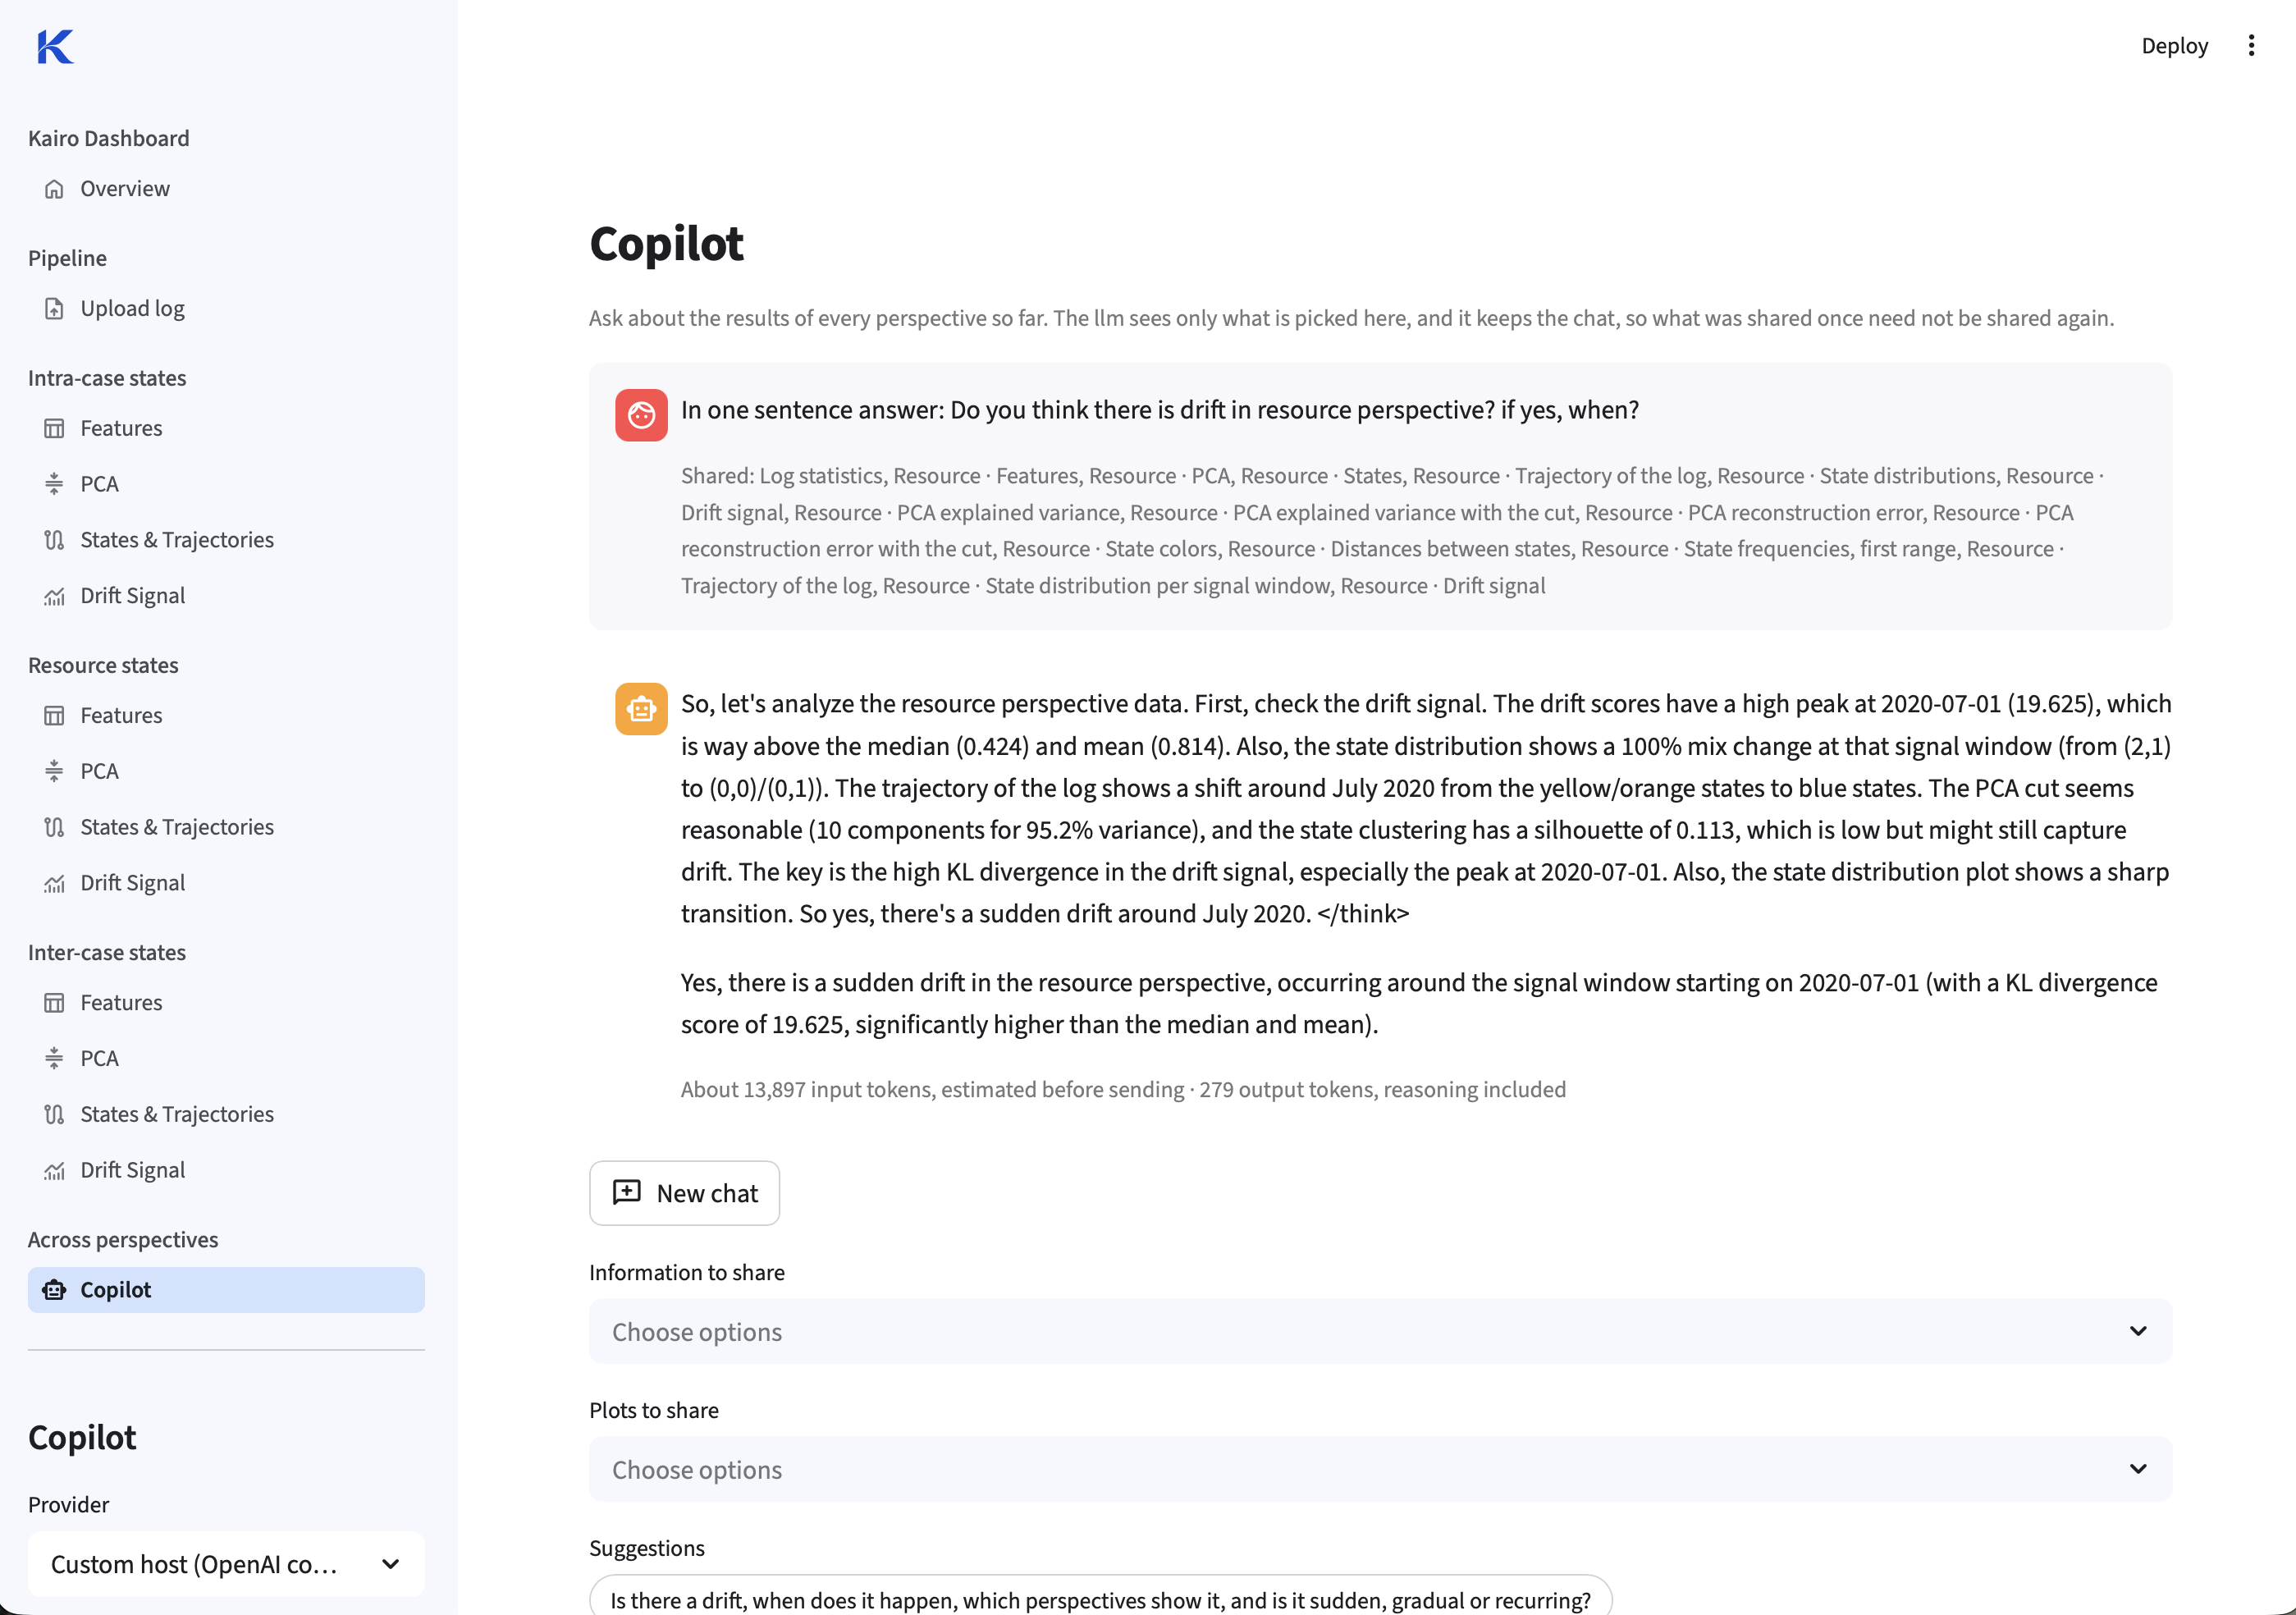
\includegraphics[width=\textwidth]{figures/dashboard/copilot}
	\caption[Copilot page of the dashboard]{%
		Copilot page of the dashboard for the resource perspective of the running example $L_3$. The user shares the log statistics as well as the abstractions and plots of all steps of the resource perspective of Figures~\ref{fig:impl:dashboard_states} to~\ref{fig:impl:dashboard_drift} and asks whether there is a drift in the resource perspective and when. The model Qwen3-VL-30B-A3B-Thinking, a custom provider in the sidebar, answers with its reasoning, which ends with \texttt{</think>}, and then names a sudden drift in the signal window from July~1, 2020.}
	\label{fig:impl:copilot}
\end{figure}
